% Chapter 1

\chapter{Introducción general} % Main chapter title

\label{Chapter1} % For referencing the chapter elsewhere, use \ref{Chapter1} 
\label{IntroGeneral}

%----------------------------------------------------------------------------------------

% Define some commands to keep the formatting separated from the content 
\newcommand{\keyword}[1]{\textbf{#1}}
\newcommand{\tabhead}[1]{\textbf{#1}}
\newcommand{\code}[1]{\texttt{#1}}
\newcommand{\file}[1]{\texttt{\bfseries#1}}
\newcommand{\option}[1]{\texttt{\itshape#1}}
\newcommand{\grados}{$^{\circ}$}

%----------------------------------------------------------------------------------------

%\section{Introducción}
En este capítulo se presentan los conceptos necesarios para comprender el método de titulación y el funcionamiento de los tituladores automáticos, así como también se realiza una exploración de trabajos de I+D y productos comerciales similares al prototipo presentado. Por último se destaca el origen de la propuesta y los objetivos y alcances del trabajo realizado.

%----------------------------------------------------------------------------------------
\section{Concepto de titulación}

La titulación es una técnica analítica que permite realizar la determinación cuantitativa de la concentración de una sustancia o grupo de sustancias químicas (analitos) en una muestra problema. Este método de análisis químico se basa en medir la cantidad de un reactivo de concentración conocida, denominado titulante, que es consumida por un analito durante una reacción química o electroquímica. En una titulación se determina el volumen o la masa de titulante necesaria para reaccionar completamente con el analito, y este dato permite calcular la cantidad del analito presente en una muestra. El punto de equivalencia de la reacción, conocido como punto final cuando es determinado de manera experimental, se puede determinar por el cambio de color en un indicador o por el cambio en una respuesta instrumental, como por ejemplo, el pH \citep{BOOK:1}.

El punto de equivalencia es el punto teórico que se alcanza cuando la cantidad de titulante añadido es químicamente equivalente a la cantidad de analito
en la muestra y no puede determinarse de manera experimental. En cambio, se puede estimar su valor en base al punto final, que se da cuando se observa una variación física asociada con la condición de equivalencia \citep{BOOK:1}.

Existen diferentes tipos de titulaciones que implican diferentes métodos de análisis. Para el caso de este trabajo se utilizaron las titulaciones del tipo ácido-base, para las cuales se utilizan el método del cambio de color de un indicador y el del cambio de potencial de un electrodo.

El cambio de color es la técnica que se utiliza actualmente de manera manual en el laboratorio  de la UTN FRSFco. La figura \ref{fig:titManualColor} describe el proceso en cual se adiciona de manera lenta el titulante en la solución a analizar y cuando se produce el cambio en el color del indicador se halla el punto final.

\begin{figure}[htbp]
	\centering
	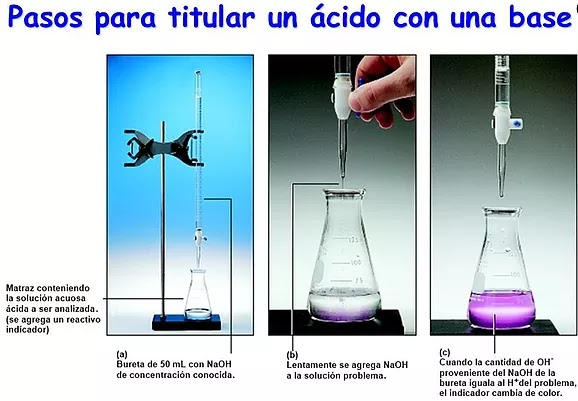
\includegraphics[width=.8\textwidth]{./Figures/titulacionManual.jpg}
	\caption{Titulación ácido-base manual mediante indicador de color\protect\footnotemark.}
	\label{fig:titManualColor}
\end{figure}



El cambio en el potencial de un electrodo de pH es la técnica que se utilizó para este trabajo y se detalla en la  figura \ref{fig:titManualPot}. En la imagen se observa un proceso manual asistido por una computadora que registra los datos de la cantidad de gotas que añade el usuario y el valor de pH leído por el electrodo.

\footnotetext{Imagen tomada de \url{https://2.bp.blogspot.com/-a9RepHphLgc/WgOVnU_U_QI/AAAAAAAAAGM/ulzSDSrbOKYNvtwqNhe_D5TE6bzxiT9aACLcBGAs/s1600/acido-base.webp}}

\begin{figure}[htbp]
	\centering
	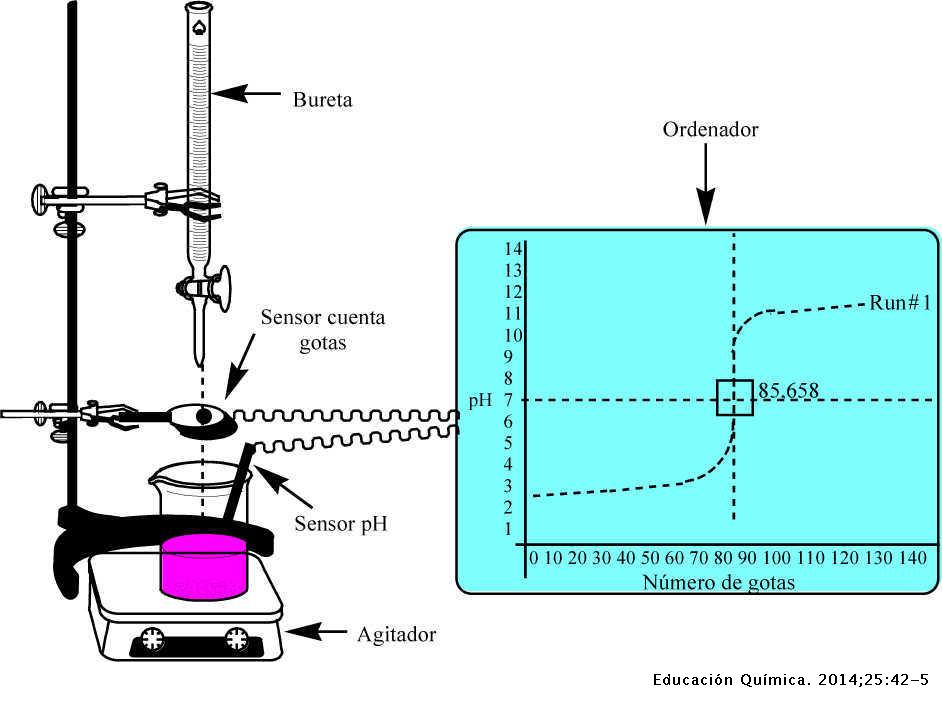
\includegraphics[width=.7\textwidth]{./Figures/titulacionPotManual.jpeg}
	\caption{Titulación ácido-base manual mediante indicador de color\protect\footnotemark.}
	\label{fig:titManualPot}
\end{figure}

\footnotetext{Imagen tomada de \url{https://www.elsevier.es/es-revista-educacion-quimica-78-articulo-titulaciones-acido-base-con-el-empleo-S0187893X14705221}}

\subsection{Curvas de titulación}

Una curva de titulación es una gráfica de alguna variable asociada a la concentración en función del volumen de titulante agregado. Generalmente se dan dos tipos de curvas: la sigmoidea y la de segmento lineal \citep{BOOK:1}.
Para el trabajo desarrollado se tuvo en cuenta la curva del tipo sigmoidea, como se muestra en la figura \ref{fig:sigmoidea}. En la misma se observa que el punto de equivalencia coincide con el punto de inflexión de la curva, característica que permite determinar de manera aproximada el punto final. 

\begin{figure}[htbp]
	\centering
	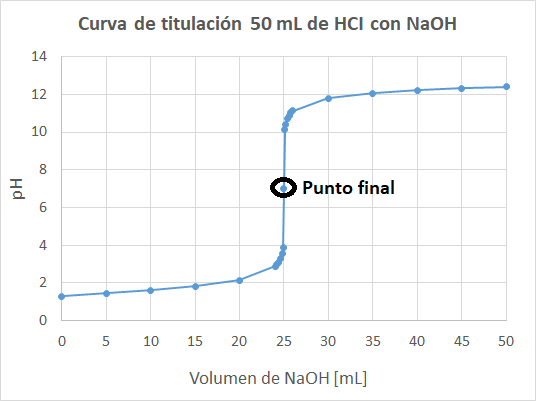
\includegraphics[width=.5\textwidth]{./Figures/curvaTitulacion1.png}
	\caption{Curva de titulación del tipo sigmoidea\protect\footnotemark.}
	\label{fig:sigmoidea}
\end{figure}

\footnotetext{Imagen tomada de \url{https://www.lifeder.com/punto-de-equivalencia/}}

\subsection{Potenciometría}

La potenciometría se basa en la medición del potencial de celdas electroquímicas  con corriente despreciable. Para llevar a cabo se utilizan dos electrodos: un electrodo de referencia con potencial conocido e independiente de la solución analizada, y un electrodo indicador cuya tensión varía en función de la actividad del analito,  separados por un puente salino que previene que los componentes de la disolución de analito se mezclen con los componentes del electrodo de referencia, tal y como se muestra en la figura \ref{fig:potenciometria} \citep{BOOK:1}.

\begin{figure}[htbp]
	\centering
	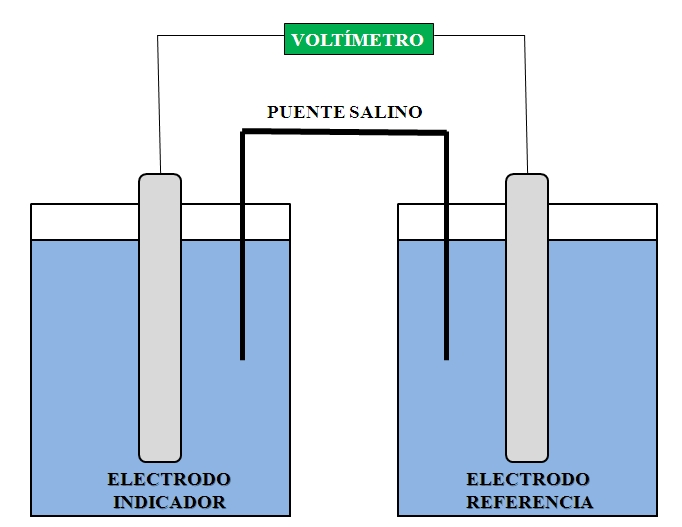
\includegraphics[width=.5\textwidth]{./Figures/Potenciometria-img.jpg}
	\caption{Curva de titulación del tipo sigmoidea\protect\footnotemark.}
	\label{fig:potenciometria}
\end{figure}

\footnotetext{Imagen tomada de \url{https://www.lifeder.com/potenciometria/}}
%----------------------------------------------------------------------------------------
\section{Descripción de tituladores automáticos}
\label{tituladoresAutomaticos}

Un titulador automático es un dispositivo que agrega titulante en la solución a analizar y registra alguna variable física por cada unidad de volumen o masa de titulante agregada. En base a esos datos, se puede elaborar la curva de titulación y calcular el volumen o masa en el punto final.
Existen diferentes tipos de tituladores que se usan para diferentes análisis, como por ejemplo el titulador potenciométrico, el de conductividad, Karl Fischer, entre otros.

Un titulador potenciométrico automático hace uso de un electrodo para medir el potencial de la celda a la vez que inyecta el titulante mediante el uso de algún sistema de dosificación, y registra cada valor potencial en mV o en pH en función de la cantidad de volumen añadido. Además, estos dispositivos suelen incluir un agitador que permite acelerar el proceso de mezcla entre el titulante añadido y la solución, para que el cambio en el potencial se visualice de manera más rápida.
En la figura \ref{fig:titThermo} se observa un ejemplo de un titulador comercial para titulaciones del tipo ácido-base.

\begin{figure}[htbp]
	\centering
	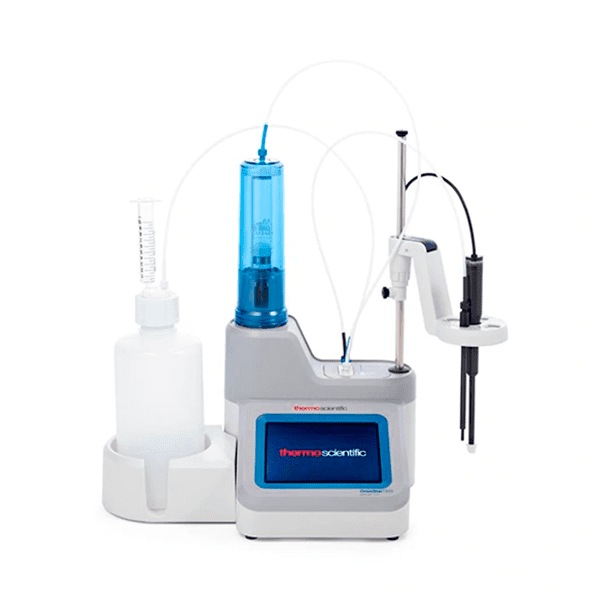
\includegraphics[width=.6\textwidth]{./Figures/titThermo.png}
	\caption{Ejemplo de titulador automático. Marca THERMO SCIENTIFIC\protect\footnotemark.}
	\label{fig:titThermo}
\end{figure}

\footnotetext{Imagen tomada de \url{https://www.equiposylaboratorio.com/portal/productos/titulador-automAtico-thermo-scientific-start9100-orion-star-t910}}



%----------------------------------------------------------------------------------------
\section{Estado del arte}

Existen gran variedad de tituladores potenciométricos automáticos en el mercado con diferentes características. La tabla \ref{tab:titComerciales} ilustra una comparativa entre algunos modelos de tituladores que disponen diferentes laboratorios de la región. \textbf{(acá podría explicar el contenido de la tabla)}

\begin{table}[h]
	\centering
	\caption[caption corto]{Comparativa de tituladores comerciales}
	\begin{tabular}{l c c}    
		\toprule
		\textbf{Marca} 	 & \textbf{Modelo} 		& \textbf{Características}  \\
		\midrule
		Kem					 & AT510 			& a \\		
		Mettler Toledo		 & Compact			& b \\
		Hanna				 & HI901C1-01		& c \\
		\bottomrule
		\hline
	\end{tabular}
	\label{tab:titComerciales}
\end{table}

%----------------------------------------------------------------------------------------
\section{Motivación}
El desarrollo de un titulador automático surgió de la iniciativa del grupo de I+D GISAI perteneciente a la UTN FRSFco con el fin de encarar un proyecto multidisciplinar en el que se involucren las cuatro carreras de ingeniería de la facultad. Luego de confirmar los integrantes del proyecto, se decidió en conjunto construir un titulador de bajo costo para el laboratorio de servicios de química, ya que los tituladores comerciales son económicamente inaccesibles para universidades y laboratorios en los que existe una frecuencia baja de muestras a analizar.
Una vez planteado el proyecto, se dividieron los objetivos particulares de cada área disciplinar, los cuales se detallan a continuación:
\begin{itemize}
\item Ingeniería Química: encargada de establecer los requerimientos y de validar el prototipo.
\item Ingeniería Electrónica: encargada de diseñar e implementar el sistema embebido que controle el proceso de titulación.
\item Ingeniería Electromecánica: encargada de diseñar y desarrollar la bomba y otros componentes mecánicos, como ca carcasa.
\item Ingeniería en Sistemas de Información: encargada de elaborar el software que procesará los datos entregados por el titulador y otros datos asociados a la muestra analizada y al cliente que lo solicita.
\end{itemize}
En esta memoria se describen las tareas realizadas dentro del área de Ingeniería Electrónica, cuyos objetivos y alcances se encuentran detallados en la sección \ref{objYalc}.

%----------------------------------------------------------------------------------------
\section{Objetivos y alcance}
\label{objYalc}

El trabajo realizado consistió en desarrollar el prototipo de un sistema embebido que permita automatizar y controlar el método de titulación potenciométrica.

El trabajo incluye:
\begin{itemize}
\item Una interfaz de usuario que permite realizar las configuraciones correspondientes, calibrar el dispositivo, y dar inicio y fin al proceso de titulación.
\item La visualización de la curva de pH respecto al tiempo.
\item El control de la bomba que inyecta el titulante en la solución a analizar.
\item El cálculo y visualización del volumen del titulante en el punto final.
\item El almacenamiento de los datos del ensayo en una memoria SD.
\item La visualización de los datos del ensayo en una página web, a través de una conexión Wi-Fi local.
\end{itemize}

El trabajo no incluye:
\begin{itemize}
\item El manejo del dispositivo de manera remota.
\item El diseño de la carcasa u otras partes mecánicas. 
\end{itemize}

En el diagrama de la figura \ref{fig:diagramaBloqueSimple} se muestra como interactúa el sistema desarrollado con las partes intervinientes. El sistema embebido es el encargado de controlar el volumen de titulante que la bomba agrega a la solución, y de leer el valor de pH obtenido por el electrodo. Una vez obtenidos todos los valores del proceso, los almacena en una tabla y calcula el volumen correspondiente al punto final. Ambos datos son enviados al software de la computadora.

\begin{figure}[htbp]
	\centering
	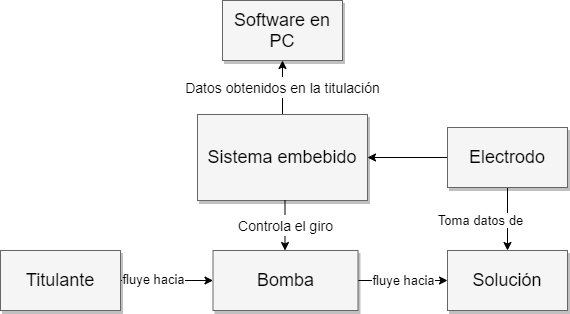
\includegraphics[width=.8\textwidth]{./Figures/DiagramaBloquesSimple.png}
	\caption{Diagrama en bloques simplificado.}
	\label{fig:diagramaBloqueSimple}
\end{figure}